\section{End-to-end comparison (accuracy pending)}
\label{sec:live}

Table~\ref{tab:main} is laid out like Table~2 of MADKE \cite{wang2025madke}. Published values are transcribed from that paper (arXiv v2) and are not re-measured; the cells marked ``--'' are empty because no model was available. They are not estimates, and nothing in this paper should be read as a prediction of them. The ``re-run'' row is needed because a published number and a number from our harness can differ in prompts, sampling and judge.

\begin{table}[!htbp]
\centering
\tiny
\caption{Main comparison protocol. F1 and GPT-4 score (G4) for generative QA, exact match for FEVER. Rows other than the two marked ones are transcribed from the base paper; ``--'' = not yet measured.}
\label{tab:main}
\setlength{\tabcolsep}{3.2pt}
\resizebox{\textwidth}{!}{%
\begin{tabular}{llccccccccc}
\toprule
Backbone & Method & TQA F1 & TQA G4 & NQ F1 & NQ G4 & HQA F1 & HQA G4 & 2W F1 & 2W G4 & FEV EM \\
\midrule
\multirow{8}{*}{GPT-3.5-Turbo}
 & SP & 0.761 & 0.778 & 0.390 & 0.532 & 0.331 & 0.384 & 0.190 & 0.210 & 0.548 \\
 & CoT & 0.715 & 0.772 & 0.418 & 0.588 & 0.333 & 0.410 & 0.165 & 0.190 & 0.556 \\
 & SC & 0.756 & 0.818 & 0.431 & 0.622 & 0.342 & 0.408 & 0.175 & 0.206 & 0.560 \\
 & RAG & 0.768 & 0.824 & 0.450 & 0.436 & 0.423 & 0.498 & 0.204 & 0.228 & 0.646 \\
 & MAD & 0.712 & 0.798 & 0.401 & 0.648 & 0.287 & 0.394 & 0.133 & 0.186 & 0.548 \\
 & MADKE (as published) & 0.728 & 0.830 & 0.453 & 0.736 & 0.405 & 0.542 & 0.205 & 0.274 & 0.612 \\
 & MADKE (re-run, our harness) & -- & -- & -- & -- & -- & -- & -- & -- & -- \\
 & \textbf{MADKE-X (ours)} & -- & -- & -- & -- & -- & -- & -- & -- & -- \\
\midrule
\multirow{8}{*}{Qwen1.5-32B-Chat}
 & SP & 0.581 & 0.632 & 0.295 & 0.462 & 0.311 & 0.384 & 0.207 & 0.220 & 0.536 \\
 & CoT & 0.587 & 0.644 & 0.276 & 0.452 & 0.315 & 0.382 & 0.220 & 0.228 & 0.546 \\
 & SC & 0.583 & 0.628 & 0.276 & 0.442 & 0.312 & 0.386 & 0.203 & 0.222 & 0.540 \\
 & RAG & 0.446 & 0.554 & 0.269 & 0.436 & 0.309 & 0.420 & 0.183 & 0.248 & 0.664 \\
 & MAD & 0.630 & 0.704 & 0.321 & 0.566 & 0.363 & 0.482 & 0.256 & 0.286 & 0.520 \\
 & MADKE (as published) & 0.763 & 0.838 & 0.475 & 0.724 & 0.450 & 0.570 & 0.258 & 0.314 & 0.646 \\
 & MADKE (re-run, our harness) & -- & -- & -- & -- & -- & -- & -- & -- & -- \\
 & \textbf{MADKE-X (ours)} & -- & -- & -- & -- & -- & -- & -- & -- & -- \\
\midrule
\multirow{8}{*}{Qwen1.5-72B-Chat}
 & SP & 0.665 & 0.706 & 0.378 & 0.550 & 0.332 & 0.428 & 0.226 & 0.260 & 0.596 \\
 & CoT & 0.715 & 0.776 & 0.406 & 0.648 & 0.431 & 0.514 & 0.275 & 0.324 & 0.625 \\
 & SC & 0.659 & 0.700 & 0.369 & 0.548 & 0.336 & 0.430 & 0.207 & 0.242 & 0.596 \\
 & RAG & 0.662 & 0.762 & 0.333 & 0.710 & 0.438 & 0.538 & 0.217 & 0.304 & 0.668 \\
 & MAD & 0.703 & 0.796 & 0.376 & 0.660 & 0.397 & 0.548 & 0.274 & 0.344 & 0.516 \\
 & MADKE (as published) & 0.787 & 0.874 & 0.479 & 0.748 & 0.495 & 0.622 & 0.284 & 0.350 & 0.686 \\
 & MADKE (re-run, our harness) & -- & -- & -- & -- & -- & -- & -- & -- & -- \\
 & \textbf{MADKE-X (ours)} & -- & -- & -- & -- & -- & -- & -- & -- & -- \\
\midrule
GPT-4-Turbo & SP (reference) & 0.828 & 0.902 & 0.459 & 0.692 & 0.472 & 0.566 & 0.265 & 0.284 & 0.608 \\
\bottomrule
\end{tabular}%
}
\end{table}

\paragraph{Planned additional analyses} (i) Knowledge source (none, Wikipedia, Google, both) with and without the evidence governor; (ii) component ablation (Section~\ref{sec:design}); (iii) model scale (Qwen1.5 1.8B--72B); (iv) number of agents and rounds on GPT-3.5-Turbo; (v) token cost against MADKE and MAD, where the published MADKE figure is 27.5\% fewer output tokens than MAD; (vi) consistent-but-wrong rate and support-status distribution, which only MADKE-X can report; (vii) a case study with a printed trace; and (viii) a human audit of 100 answers for GPT-4-score agreement.

\begin{figure}[!htbp]
\centering
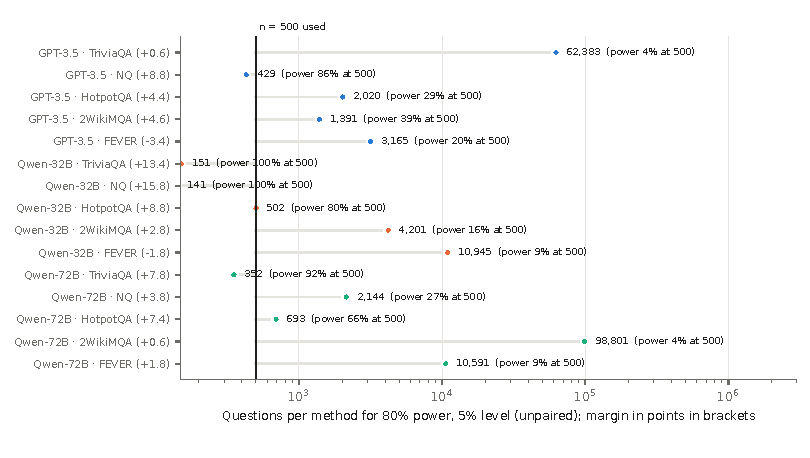
\includegraphics[width=\textwidth]{fig6_power}
\caption{Questions needed for 80\% power at each published margin; the line marks $n{=}500$. Differences below roughly 5 points are not resolvable per dataset at this size.}
\label{fig:power}
\end{figure}
